\documentclass[mat2, tisk]{fmfdelo}
% \documentclass[fin2, tisk]{fmfdelo}
% \documentclass[isrm2, tisk]{fmfdelo}
% \documentclass[ped, tisk]{fmfdelo}
% Če pobrišete možnost tisk, bodo povezave obarvane,
% na začetku pa ne bo praznih strani po naslovu, …
%%%%%%%%%%%%%%%%%%%%%%%



%%%%%%%%%%%%%%%%%%%%%
%%%%%%%%%%%%%%%%%%%%%%%%%%%%%%%%%%%%%%%%%%%%%%%%%%%%%%%%%%%%%%%%%%%%%%%%%%%%%%%
% METAPODATKI
%%%%%%%%%%%%%%%%%%%%%%%%%%%%%%%%%%%%%%%%%%%%%%%%%%%%%%%%%%%%%%%%%%%%%%%%%%%%%%%

% - vaše ime
\avtor{Urh Primožič}

% - naslov dela v slovenščini
\naslov{Iskanje morfizmov z gradientnim spustom}

% - naslov dela v angleščini
\title{Finding morphisms with gradient
descent}

% - ime mentorja/mentorice s polnim nazivom:
%   - doc.~dr.~Ime Priimek
%   - izr.~prof.~dr.~Ime Priimek
%   - prof.~dr.~Ime Priimek
%   za druge variante uporabite ustrezne ukaze
\mentor{prof.~dr.~Ljupčo Todorovski}
\somentor{doc.~dr.~Urban Jezernik}
% \mentorica{...}
% \somentorica{...}
% \mentorja{...}{...}
% \somentorja{...}{...}
% \mentorici{...}{...}
% \somentorici{...}{...}

% - leto magisterija
\letnica{2025}

% - povzetek v slovenščini
%   V povzetku na kratko opišite vsebinske rezultate dela. Sem ne sodi razlaga
%   organizacije dela, torej v katerem razdelku je kaj, pač pa le opis vsebine.
\povzetek{Tukaj napišemo povzetek vsebine. Sem sodi razlaga vsebine in ne opis tega, kako je delo organizirano.

  }

% - povzetek v angleščini
\abstract{An abstract of the work is written here. This includes a short description of
the content and not the structure of your work.}

% - klasifikacijske oznake, ločene z vejicami
%   Oznake, ki opisujejo področje dela,\textbf{} so dostopne na strani https://www.ams.org/msc/


% 15A69	Multilinear algebra: matrix/tensor parameterization
% 20C30	Representations of symmetric and related finite groups
% 20C99	Group representation aspects not covered elsewhere
% 68T05	Machine learning: gradient-based learning systems
% 65K10	Numerical optimization: gradient descent and variational methods
% 68T09	AI methods in symbolic group computation


\klasifikacija{65K10, 68T05, 20C99, 68T09}

% - ključne besede, ki nastopajo v delu, ločene s \sep
\kljucnebesede{gradientni spust\sep upodobitve\sep izomorfizmi grafov\sep delovanja\sep grafovske nevronske mreže
% \texorpdfstring{$C^*$}{C*}-algebre
}

% - angleški prevod ključnih besed
\keywords{
gradient descent\sep representations\sep graph isomorphisms\sep actions\sep graph neural networks
}

% - neobvezna zahvala
\zahvala{
  Neobvezno.
  Zahvaljujem se \dots
}

% - ime datoteke z viri (vključno s končnico .bib), če uporabljate BibTeX
\literatura{literatura.bib}

%%%%%%%%%%%%%%%%%%%%%%%%%%%%%%%%%%%%%%%%%%%%%%%%%%%%%%%%%%%%%%%%%%%%%%%%%%%%%%%
% DODATNE DEFINICIJE
%%%%%%%%%%%%%%%%%%%%%%%%%%%%%%%%%%%%%%%%%%%%%%%%%%%%%%%%%%%%%%%%%%%%%%%%%%%%%%%

% naložite dodatne pakete, ki jih potrebujete
\usepackage{pdfpages}
\usepackage{units}        % fizikalne enote kot \unit[12]{kg} s polovico nedeljivega presledka, glej primer v kodi
\usepackage{graphicx}     % za slike
\usepackage{subcaption}
% \usepackage{pgffor}
\usepackage{tikz}
\usepackage{etoolbox}
\usepackage{xparse} 
% \usepackage{tikz}
% VEČ ZANIMIVIH PAKETOV
% \usepackage{array}      % več možnosti za tabele
% \usepackage[list=true,listformat=simple]{subcaption}  % več kot ena slika na figure, omogoči slika 1a, slika 1b
% \usepackage[all]{xy}    % diagrami
% \usepackage{doi}        % za clickable DOI entrye v bibliografiji
% \usepackage{enumerate}     % več možnosti za sezname

% Za barvanje source kode
% \usepackage{minted}
% \renewcommand\listingscaption{Program}

% Za pisanje psevdokode
% \usepackage{algpseudocode}  % za psevdokodo
% \usepackage{algorithm}
% \floatname{algorithm}{Algoritem}
% \renewcommand{\listalgorithmname}{Kazalo algoritmov}

% deklarirajte vse matematične operatorje, da jih bo LaTeX pravilno stavil
% \DeclareMathOperator{\...}{...}

% vstavite svoje definicije ...
%%%%%%%%%%%%%%%%%%%
% MOJE DEFINICIJE
%%%%%%%%%%%%%
% \fortable{n}{begin}{end}{n_columns}{column} naredi tabelo 
\newcommand{\TODO}[1]{{\color{blue} TODO: #1}}
\newcommand{\R}{\mathbb R}
\newcommand{\N}{\mathbb N}
\newcommand{\Z}{\mathbb Z}
\newcommand{\loss }{\mathcal L}
\newcommand{\fun}{\operatorname{fun}}
\newcommand{\funnn}[1]{\fun([#1], [#1])}
\newcommand{\Loss}[1]{\mathcal L _\text{#1}}
% Lahko se zgodi, da je ukaz \C definiral že paket hyperref,
% zato dobite napako: Command \C already defined.
% V tem primeru namesto ukaza \newcommand uporabite \renewcommand
\newcommand{\C}{\mathbb C}
\newcommand{\Q}{\mathbb Q}

%%%%%%%%%%%%%%%%%%%%%%%%%%%%%%%%%%%%%%%%%%%%%%%%%%%%%%%%%%%%%%%%%%%%%%%%%%%%%%%
% ZAČETEK VSEBINE
%%%%%%%%%%%%%%%%%%%%%%%%%%%%%%%%%%%%%%%%%%%%%%%%%%%%%%%%%%%%%%%%%%%%%%%%%%%%%%%

\begin{document}

\section{Uvod}
Napišite kratek zgodovinski in matematični uvod.  Pojasnite motivacijo za problem, kje
nastopa, kje vse je bil obravnavan. Na koncu opišite tudi organizacijo dela -- kaj je v
katerem razdelku.

Motivacija: iskanje diskretnih struktur v matematiki (upodobitev, delovanj, izomorfizmov grafov). Razvoj in uspeh gradientnih metod. Iskanje morfizmov z gradientnimi metodami. 

Zgodovina: Izračunljivost in časovna zahtevnost determinističnih metod. Uporaba ml do zdaj. 

Originalni rezultati: Naši izsledki. Isti setup za vse tri stvari. Implementacija. 

Struktura: \TODO{dopiši na koncu}


\section{Optimizacija z gradientnim spustom}
Na različne probleme v matematiki lahko gledamo kot na iskanje minimuma $\hat \phi = \operatorname{argmin}( \mathcal L(\phi) \mid  \phi )$ nekega funckionala. Če je domena funkcionala evklidski prostor, $\mathcal{L}\colon \R^n \to \R$ pa gladka, lahko minimum iščemo z gradientnimi metodami optimizacije.

\begin{primer}
    \TODO{ Ali dodam kak primer?}
\end{primer}

    \subsection{Gradientni spust}
   \begin{definicija}
   \TODO{VPRAŠANJE: kateri vir vzamem za gradient descent?}
       Naj bo $\mathcal{L} \colon \R^n  \to \R$ odvedljiva funkcija in $\phi_0 \in \R^n$ poljubna začetna vrednost parametrov. \emph{Gradientni spust}\index{gradientni spust} je iterativna optimizacijska metoda, definirana s pravilom
       \begin{equation}
            \label{eq:gradientni spust}
            \phi_{i+1} = \phi_i - \eta \nabla \mathcal{L}(\phi_i)
       \end{equation}
       Parametru
       $\eta > 0$ rečemo   hitrost učenja (\emph{learning rate}) gradientnega spusta in vpliva na velikost spremembe parametrov.
        \end{definicija} 



\begin{primer}
Na sliki~\ref{fig:primer gradientnega spusta} sta prikazana grafa rezultatov gradientnega spusta na funkciji $f(x) = x e^{\sqrt{x} - 2x\sin(x)}$ z začetnim parametrom $x_0 = 1$ in različnima hitrostima učenja. Spremembe parametrov sledijo smeri padanja krivulje in so večje, če krivulja pada hitreje. 
           \begin{figure}[ht]
  \centering
  \includegraphics[width=0.9\textwidth]{images/im:gradient_descent_example.pdf}
  \caption[Primer delovanja gradientnega spusta.]{$100$ korakov gradientnega spusta na funkciji $f(x) = x e^{\sqrt{x} - 2x\sin(x)}$ z začetnim parametrom $x_0=1$ in hitrostjo učenja $\eta$. V obeh primerih metoda konvergira do lokalnega minimuma funkcije, ki ni globalni. }
  \label{fig:primer gradientnega spusta}
\end{figure}
\end{primer}

       


    
  
        \subsubsection{Gradientni tok}
        \index{gradientni tok}
        Naj bosta $\mathcal{L}$ in $\phi$ kot zgoraj. \emph{Gradientni tok} je rešitev diferencialne enačbe
        \begin{equation}
            \label{eq:gradient flow}
            \frac{d\phi}{d t} = - \nabla \mathcal{L}(\phi), \quad \phi(0)=\phi_0.
        \end{equation}
        
        Gradientni spust je ekvivalenten numeričnem reševanju diferencialne enačbe \emph{gradientnega toka} z Eulerjevo metodo \TODO{dodaj vir!}. 

    \subsection{Lastnosti gradientnega spusta}
    V primeru~\ref{fig:primer gradientnega spusta} metoda konvergira do lokalnega minimuma funkcije. Konvergence do globalnih ekstremov očitno ne moremo pričakovati, velja pa za konveksne funkcije (\TODO{članek}). Konvergenco do globalnega minimuma lahko dosežemo tudi z prekomerno parametrizacijo (\emph{overparametrisation \TODO{članki do teh izrekov}}.

    Metoda ne konvergira vedno. 
    
    \subsection{Adam}
    \index{adam}
        \TODO{Motivacija, lastnosti, definicija}
    \subsection{Nevronske mreže}
    \subsection{Grafovske nevronske mreže}
\section{Iskanje upodobitev}
    \subsection{Upodobitve končnih grup}
    \begin{definicija}
    \index{upodobitev}
        Naj bo $G$ grupa in $V$ vektorski prostor nad poljem $\mathbb{F}$. \emph{Upodobitev grupe $G$} je homomorfizem $ \rho \colon G \to \operatorname{GL(V)}$ med grupo $G$ in endomorfizmi prostora $V$.
    \end{definicija}
    Vsaka upodobitev $\rho \colon G \to \operatorname{GL}(V)$ naravno definira linearno delovanje $v ^ g = \rho(g)(v)$ grupe nad $V$. Ekvivalentno vsako linearno delovanje  definira upodobitev $\rho(g) = (v \mapsto v^g)$. 
    \begin{definicija}
        Upodobitvi $\rho \colon G \to \operatorname{GL}(V)$ in 
         $\sigma \colon G \to \operatorname{GL}(W)$ sta \emph{ekvivalentni}, če obstaja izomorfizem vektorskih prostorov $\Phi \colon  V \to W$, da za vsak $g \in G$ in vsak $v \in V$ velja 
         $$
         \Phi(\rho(g)(v)) = \sigma(g)(\Phi(v)).
         $$
         Preslikavi $\Phi$ rečemo \emph{spletična} med $V$ in $W$.
    \end{definicija}
    \begin{definicija}
        Naj bo $\rho: G \to \operatorname{GL}(V)$ upodobitev in $W < V$ podprostor prostora $V$, invarianten za inducirano delovanje. Potem je upodobitev
        $
        \rho_W \colon G \to \operatorname{GL(W)}
        $, dana s predpisom
        $\rho_W(g) = \rho(g)|_{W}$ \emph{podupodobitev} upodobitve $\rho$.
    \end{definicija}
    \begin{definicija}
    \index{nerazcepna upodobitev}
        Če sta edini podupodobitvi upodobitve $\rho \colon G \to \operatorname{GL}(V)$ $g \mapsto \operatorname{id}$ in $\rho$, je $\rho$ \emph{nerazcpena upodobitev}. 
        Množico nerazcepnih upodobitev grupe $G$ označimo z $\operatorname{Irr}(G)$.
    \end{definicija}
    \begin{definicija}
        Upodobitev $\rho \colon G \to \operatorname{GL}(V)$ je \emph{polenostavna}, če jo lahko izrazimo kot vsoto nerazcpenih upodobitev $\rho = \bigoplus _{i \in I} \rho_i$. 
    \end{definicija}
    Če se omejimo le na končne grupe in dovolj lepa polja, so vse upodobitve sestavljene iz nerazcepnih.
    \begin{izrek}%{Polenostavnost upodobitev}
        Naj bo $G$ končna grupa in $\mathbb{F}$ 
        polje. Vse upodobitve $G$ nad poljem $F$ so polenostavne če in samo če $\operatorname{char}F \nmid |G|$.
    \end{izrek}
\begin{izrek}
    Naj bo $G$ končna grupa in $\rho \colon G \to \operatorname{GL}(V)$ končno-razsežna upodobitev nad algebraično zaprtim poljem s karakteristiko $0$. Potem velja 
    \begin{equation}
        \label{eq:nerazcepna iff norma=1}
        \rho \in \operatorname{Irr}(G) \iff |\chi_\rho| = \frac{1}{|G|} 
    \sum\limits_{g \in G} \operatorname{tr}(\rho(g)) \operatorname{tr}(\rho(g^{-1}) = 1.
    \end{equation}
\end{izrek}
    Za študij upodobitev končnih grup nad ugodnimi polji je torej dovolj poznati le končno \footnote{TODO dodaj vir} množico nerazcepnih upodobitev $\operatorname{Irr}(G) = \{ \rho \colon G \to \operatorname{GL}(V) \mid |\chi_\rho| = 1\}$.
    \subsection{Iskanje upodobitev z gradientnim spustom}
    Naj bo $G=<S|R>$ končna grupa nad množico generatorjev $S$, definirana z relacijami $R$. Na $S$ definiramo poljubno preslikavo
    \begin{align}
    \label{eq: repr model na S}
    \hat \rho \colon S &\to \C^{n \times n}    \\
    s &\mapsto 
        \begin{bmatrix}
        s_{1,1} & \cdots & s_{1,n} \\
        \vdots & & \vdots \\ 
        s_{n,1} & \cdots & s_{n,n}
    \end{bmatrix},
    \end{align}
    ki vsak generator grupe preslika v poljubno matriko. 
    Preslikavo $\hat \rho$ implicitno razširimo na celo grupo. Za generator $s \in S$ nastavimo $\hat \rho(s^{-1}) = \hat\rho(s)^{-1}$, za poljuben produkt elementov $s_1, s_2, \dotsc, s_n \in S \cup S^{-1}$
    pa definiramo
    \begin{equation}
        \label{eq: implicitna definicija upodovbitve}
        \hat \rho(s_1 s_2 \dotsm s_m) = \hat\rho(s_1)\hat\rho(s_2) \dotsm \hat\rho(s_m).
    \end{equation}
    Preslikava $\hat \rho$ ni nujno upodobitev, služi pa nam lahko kot model upodobitve, odvisen od parametrov $\phi = \{s_{i,j} \mid s \in S, 1 \leq i, j \leq n\}$.
    Parametre matrik $\hat\rho(s)$ bomo postopoma spreminjali s gradientnim spustom, da bo model vse bližje upodobitvi.

    \subsubsection{Funkcija izgube nad relacijami}
    \label{funckija izgube nad relacijami}
    Preslikava $\hat \rho$ je homomorfizem natanko tedaj, ko za vsako relacijo $r \in R$ velja 
    $
    \hat \rho(r) = I 
    $. Manjše, kot so norme $||\hat \rho(r) - I ||_F$, bolj je model $\hat\rho$ podoben homomorfizmu. 
    \begin{definicija}
        \emph{Funkcija izgube nad relacijami} je definirana kot 
        \begin{equation}
            \label{eq:funkcija izgube nad relacijami            }
           \Loss{rel}(\hat\rho) = \frac{1}{|R|} \sum \limits_{r \in R}  ||\hat \rho(r) - I  ||_F^2.
        \end{equation}
    \end{definicija}
    Očitno je model $\hat \rho$ upodobitev natanko tedaj, ko je $ \Loss{rel}(\hat\rho) =0$.
    \begin{primer}
        Poglejmo si model $\hat \rho \colon S_3 \to \R$ eno dimenzijske realne upodobitve permutacijske grupe na treh točkah za prezentacijo $S_3 = <(12), (13)\mid (12)^2=(13)^2=(13)^{(12)}(12)^{(13)}=1>$. Model je definiran z vrednostmima 
        $\hat\rho((12)) = x$ in $\hat\rho((13)) = y$.

        Edini enodimenzionalni upodobitvi $S_3$ sta identiteta $\operatorname{id}$ in predznak permutacije $\operatorname{sign}$. Na sliki so  \ref{fig:trajektorije S3 to R} trajektorije gradientnega spusta pri optimizaciji $\Loss{rel}$ za različne začetne parametre $(x_0, y_0)$. Opazimo, nekatere trajektorije konvergirajo  do $\operatorname{id}$ nekatere do$\operatorname{sign}$, nekatere do modela, ki ni upodobitev. V tem primeru je gradientni spust našel lokalni ekstrem funkcije izgube, ki ni globalni.
        \begin{figure}[h]
  \centering
  \includegraphics[width=0.6\textwidth]{images/trajektorije_S3_to_R.pdf}
% \caption[caption za v kazalo]{Dolg caption pod sliko}
  \caption[Trajektorje učenja modela $S_3 \to \R$.]{Različne trajektorije učenja modela $\hat\rho \colon S_3 \to \R$. Začetni parametri vplivajo na uspeh optimizacije in končno upodobitev. }
  \label{fig:trajektorije S3 to R}
\end{figure}
    \end{primer}
    \begin{opomba}
        Model bi lahko definirali na celi grupi kot $\hat\rho(g)=\begin{bmatrix}
            g_{i,j}
        \end{bmatrix}_{i,j=1,\dotsc, n}$, za parametre pa vzeli elemente matrik $\hat\rho(g)$. V tem primeru je model  homomomorfizem, če $\forall g, h \in G. \hat\rho(gh)=\hat\rho(g) \hat\rho(h)$. Za funkcijo izgube lahko vzamemo
        $$
        \Loss{homo} = \frac{1}{|G|^2}\sum_{i=1}^n \sum_{j=1}^n || \hat\rho(gh)-\hat\rho(g) \hat\rho(h)||_F^2.
        $$
        in iskanje upodobitev spet prevedemo na optimizacijski problem.

        Ta pristop ni praktičen, saj privede do velikega števila parametrov $N=|G|^n$. Model upodobitve permutacijske grupe $S_n$ bi tako imel $(n!)^2$ parametrov, kar je neugodno za numerične simulacije. Če pa sledimo pristopu s prezentacijami in vzamemo minimalno množico generatorjev (recimo tranzpozicija in $n$-cikel), operiramo le s štirimi kompleksnimi parametri, neodvisno od velikosti grupe.
    \end{opomba}
     \subsubsection{Funkcija izgube za nerazcepnost}
     Iščemo lahko le nerazcepne upodobitve. Vemo že (izrek \ref{eq:nerazcepna iff norma=1}), da je upodobitev $\rho$ nerazcepna, če je norma njenega \emph{karakterja} $\chi_\rho$ enaka 1. 

     \begin{definicija}
     Definiramo funkcijo izgube za nerazcepnost
     \begin{equation}
         \label{eq:irr loss}
         \Loss{irr}(\rho) = (|\chi_\rho| - 1)^2.
     \end{equation}    
     \end{definicija}
     Za poljuben model $\hat \rho$ lahko z gradientnim pustom minimaliziramo funckijo izgube $\Loss{rel} + \Loss{irr}$ in iščemo \emph{nerazcepne} upodobitve. 
     \subsubsection{Funkcija izgube za unitarnost}
     Dodatno lahko zahtevamo, da naš model slika v unitarne matrike. Velja namreč, da je vsaka upodobitev ekvivalentna upodobitvi v unitarne matrike. \TODO{vir}
     S tem zmanjšamo število različnih upodobitev, h katerimi lahko konvergiramo. 
     \begin{definicija}
         Funkcija izgube za unitarnost je 
         \begin{equation}
             \label{eq: unitary loss}
             \Loss{unitary} = \frac{1}{|S|} \sum \limits_{s \in S} ||\hat\rho(s) \hat\rho(s)^H - I||.
         \end{equation}
     \end{definicija}
     Če ne piše drugače, od tu naprej vedno privzamemo, da minimiziramo funkcijo izgube $\loss = \Loss{rel} + \Loss{irr} + \Loss{unitary}$. Globalni minimumi te funkcije so natanko unitarne nerazcepne upodobitve.
     \subsubsection{Gradientni tok}
     \TODO{nekaj o analitičnosti rešljivosti teh enačb (težko rešljive, zato delamo le simulacije)}
    \subsection{Ciklične grupe}
    Oglejmo si naš pristop iskanja nerazcepnih upodobitev na cikličnih grupah $C_n = <z | z^n=1>$. Edine nerazcepne upodobitve ciklične grupe so 
    $$
    \rho_k(z) = e^\frac{2 \pi k}{n},
    $$
    kjer je $k \in \{0, 1, \dotsc, n\}$. Pri iskanju teh upodobitev z gradientnim spustom se bomo omejili na enodimenzionalne modele.
    
    Model $\hat\rho \colon G \to \C^*$ je določen z vrednostjo $\hat\rho(z) = x + iy$ in je odvisen od dveh realnih parametrov $x, y$. 

    Funkcije izgube so
    
    \begin{align}
        \label{eq:loss function Cn}
        \Loss{rel} &= |(x + iy)^n -1|^2\\
        \Loss{irr} &= (\frac{1}{n} \sum_{i=0}^{n-1} |(x + iy)^i|^2 -1)^2 \\
        \Loss{unitary} &= | x^2 + y^2 -1|^2.
        \end{align}
Na grafu \ref{fig:ciklicna-trajektorije} so trajektorije rešitev diferencialne enačbe $\frac{d(x,y)}{dt} = -\nabla \loss$ za različne začetne parametre, izračunane s pomočjo gradientnega spusta. Opazimo, da vse rešitve konvergirajo do nerazcepnih upodobitev. Ta rezultat teoretično podpremo v \TODO{ref}\ref{TODO}.
        \begin{figure}[ht]
            \centering
            \includegraphics[width=0.7\linewidth]{images/C3 trajektorije.pdf}
            \caption{Rešitve $\frac{d(x,y)}{dt} = -\nabla \loss$ pri različnih začetnih parametrih $(x_0, y_0)$.}
            \label{fig:ciklicna-trajektorije}
        \end{figure}
        \TODO{ostalo}
    \subsection{Redukcija funkcij izgube}
    Nerazcepne upodobitve $\rho_k$ so edine enodimenzionalne upodobitve cikličnih grup. Za poljubno upodobitev $\rho \colon C_n \to \C^*$ mora namreč veljati $1 = \rho(z^n) = \rho(z)^n$, iz česar sledi, da je $\rho = \rho_k$ za nek $k$. 
    Zato lahko pri iskanju nerazcepnih upodobitev z gradientnim spustom izpustimo $\Loss{irr}$. 
    

    Ker so vse upodobitve $\rho_k$ unitarne, lahko iz funkcije izgube izpustimo tudi $\Loss{unitary}$ in za funkcijo izgube $\loss$ vzamemo le $\loss=\Loss{rel}$.

    V splošnem lahko pri optimizaciji funkcije izgube pričakujemo lokalne minimume, v katerih je vrednost $\loss$ neničelna. Edine privlačne točke enačbe $\frac{d(x,y)}{dt} = -\nabla ||(x + iy)³n -1||^2$ pa so koreni enote $z^n=1$, torej natanko unitarne nerazcepne upodobitve.  

    \TODO{Ali dodam nekam še osnove dinamike? Ali je to očitno...}
    
    \begin{izrek}
    Edini lokalni ekstremi preslikave $(x,y) \mapsto ||(x + iy)^n -1||^2$ so $e^\frac{2 \pi i k}{n}$  za $k \in \{0,1, \dotsc, n-1\}$ in $(0,0)$. Točka $(0,0)$ je odbojna točka, ostale pa privlačne. 
    \end{izrek}
    \begin{dokaz}
        Lokalni ekstremi funkcije $\Loss{rel}$ so natanko v ničlah njenega gradienta $\nabla \Loss{rel} = (\frac{d\Loss{rel}}{dx}, \frac{d\Loss{rel}}{dy})$. 

        Uvedemo $z = x + iy$.
        % 
        \footnote{Imaginarno število $i$ v tem primeru predstavlja index.
        Zanima nas gradient $\nabla \loss \in \R^2$. Za lažje računanje $\R^2$ identificiramo z $\C$. 
        Za $u   \in \R$  $iu$ predstavlja točko $(0, u) \in \R^2$. Zato pri izpeljavi $\frac{d\loss}{dy}$ izpustimo $i$.}
        % 
        Velja $\loss = \Loss{rel} = (z^n-1)(\overline{z}^n-1)$,
        $$\frac{d\Loss{rel}}{dx} = nz^{n-1}(\overline{z}^n -1) + (z^n -1) n \overline{z}^{n-1} = 2 \operatorname{Re}(n z^{n-1}(\overline{z}^n -1))
        $$
        in 
        $$\frac{d\Loss{rel}}{dy} = 
        2\operatorname{Im}(n z^{n-1}(\overline{z}^n -1))
        $$. 
            Če velja $\nabla \loss = 0$, je $z^{n-1}(\overline{z} ^n -1) = 0$. Take vrednosti $z$ so natanko $x=y=0$ in $x + iy = e^\frac{2 \pi i k}{n}$ za $k \in \N$.

            \TODO{$0$ odbojna. (hessian >0?)}
    \end{dokaz}

    \subsection{Diederske grupe}
    Opazujmo diedersko grupo $D_n = <r, s|r^n=s^2 = (rs)^2 = 1>$. Enorazsežne upodobitve diedrske grupe so
            \begin{align*}
            \chi_{\varepsilon, \delta} \colon \quad 
            s &\mapsto \varepsilon, \\
            r &\mapsto \delta,
        \end{align*}
        kjer je  \( \varepsilon \in \{-1, 1\} \), in $\delta \in \{1, -1^{n + 1}\}$.
Dvorazsežne nerazcepne upodobitve so 
         \begin{align*}
            \rho_k \colon  s &\mapsto \begin{bmatrix}
                0 & 1 \\
                1 & 0
            \end{bmatrix}\\
            r &\mapsto \begin{bmatrix}
                \cos\left(\frac{2\pi k}{n}\right) & -\sin\left(\frac{2\pi k}{n}\right) \\
                \sin\left(\frac{2\pi k}{n}\right) & \cos\left(\frac{2\pi k}{n}\right),
            \end{bmatrix}
        \end{align*}
        kjer je $0 \leq k < \frac{n}{2} $. Vse nerazcepne upodobitve so realne, zato jih bomo iskali z realnimi modeli.
        \subsubsection{Enodimenzionalne upodobitve}
        Model enorazsežne upodobitve diedrske grupe 
        je določen s slikama generatorjev\footnote{Izrabljamo notacijo in z $r$ označimo abstraktni element grupe $D_n$ in realno število $r \in \R$, ki predstavlja sliko generatorja $r$.}
        % 
        $\hat \rho(s) = s \in \R, \hat \rho(r)=r \in \R$. Funkcije izgube so enake
        \begin{align*}
            \Loss{rel} &= \frac{1}{3} \left( |s^2 -1|^2 + |r^n -1|^2  + |(rs)^2 -1|^2  \right )\\
            \Loss{unit} &=  \frac{1}{2} \left ( |r^2 -1|^2 + |s ^2 -1|^2  \right)  \\
            \Loss{irr} &= \left ( \frac{1}{2n}\sum_{i=0}^n(|r^i|^2 + |r^is|^2)    - 1\right )^2.
        \end{align*}
        \paragraph{Numerične rešitve}
        Numerično rešujemo enačbo gradientnega toka 
        $$\frac{d(r,s)}{dt} = -\nabla(\Loss{rel} + \Loss{unit} + \Loss{irr}).$$ Za reševanje NDE uporabimo \verb|scipy.solve_ivp()|. Implementacija simulacije je v \TODO{dodatek?}. 

        Na sliki \ref{fig:Dn-trajektorije-demo} so različne rešitve enačb gradientnega toka za $n\in \{1,2,7,8\}$. Modre v limiti dosežejo ničelno funkcijo izgube. Za sod $n$ vse narisane trajektorije konvergirajo do nerazcepne upodobitve, za lih $n$ pa gradientni spust iz $[-1,0]\times[-1,1]$ nikoli ne doseže ničelne napake. Enake lastnosti opazimo na širši množici diedrskih grup - glej \TODO{grafi za ostalo} 
        
        \TODO{to je od -1 do 1. zanimiv bi blo vift, kaj se zgodi, če to razširimo!}.
        \begin{figure}[h!]
            \centering
                        \begin{minipage}{0.49\textwidth}
                            \centering
                            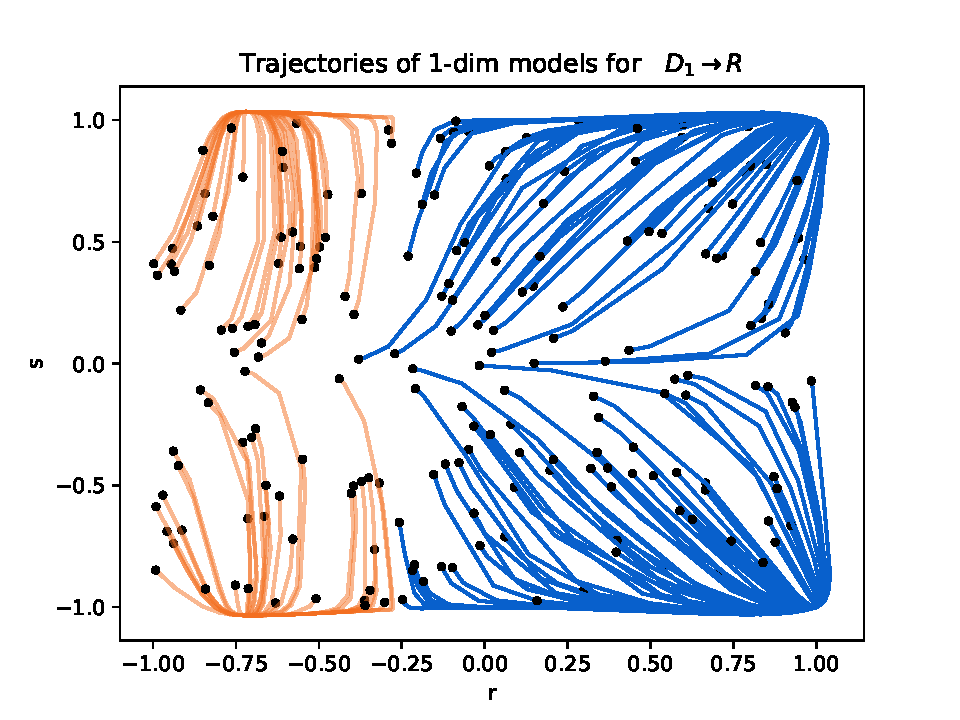
\includegraphics[width=\linewidth]{images/dihedral/Dn_1dim_n1.pdf}
                            \caption*{$n=1$}
                        \end{minipage} 
            \centering
                        \begin{minipage}{0.49\textwidth}
                            \centering
                            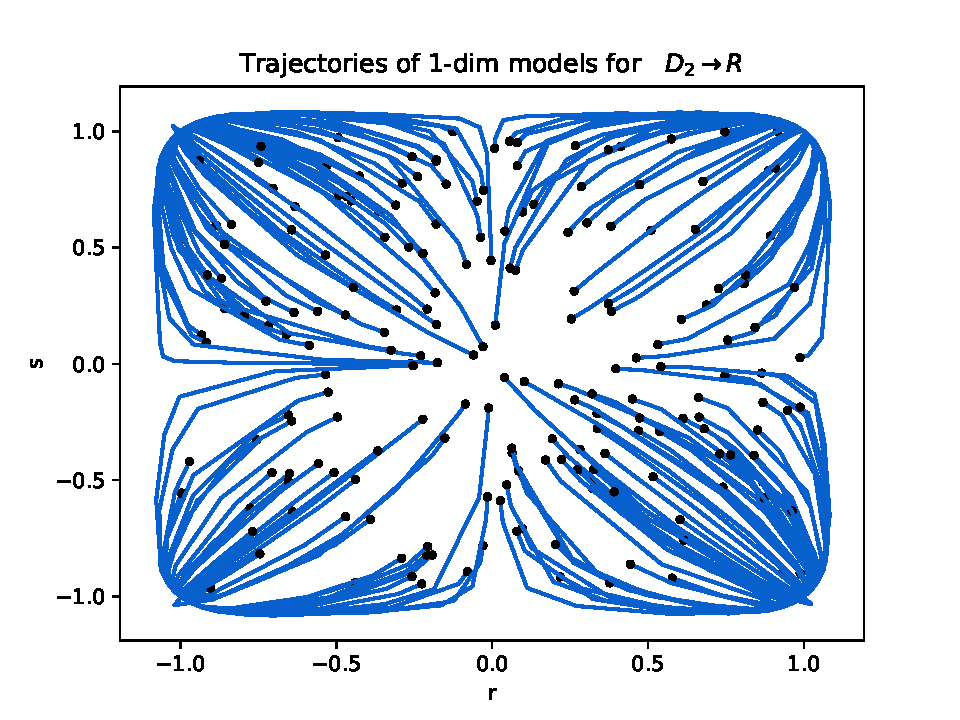
\includegraphics[width=\linewidth]{images/dihedral/Dn_1dim_n2.pdf}
                            \caption*{$n=2$}
                        \end{minipage} 
            \vspace{0.5em}
            \centering
                        \begin{minipage}{0.49\textwidth}
                            \centering
                            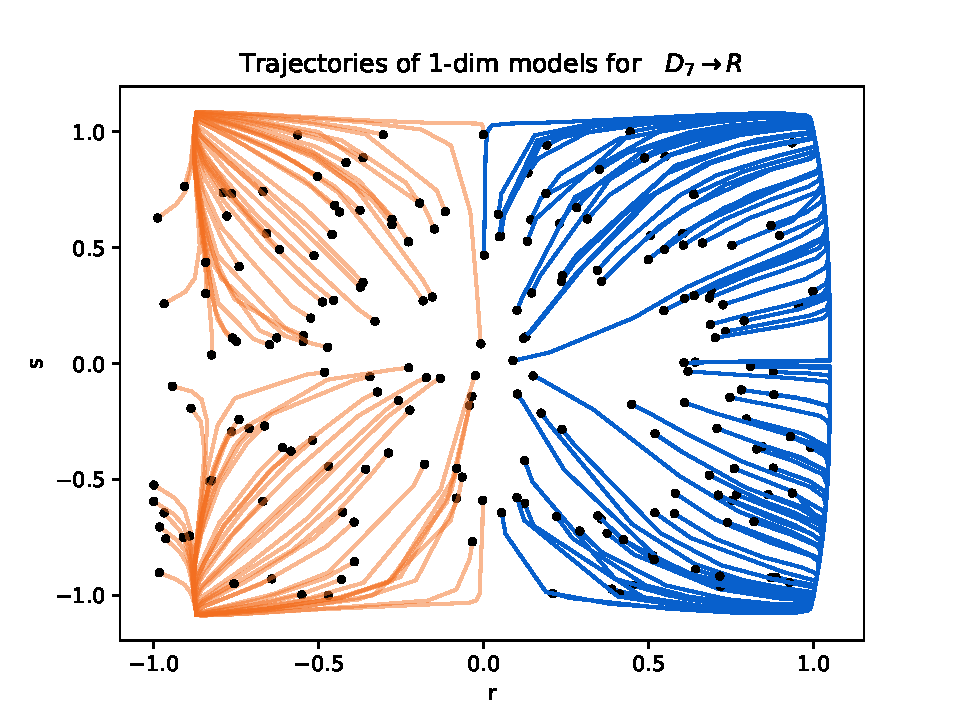
\includegraphics[width=\linewidth]{images/dihedral/Dn_1dim_n7.pdf}
                            \caption*{$n=7$}
                        \end{minipage} 
            \centering
                        \begin{minipage}{0.49\textwidth}
                            \centering
                            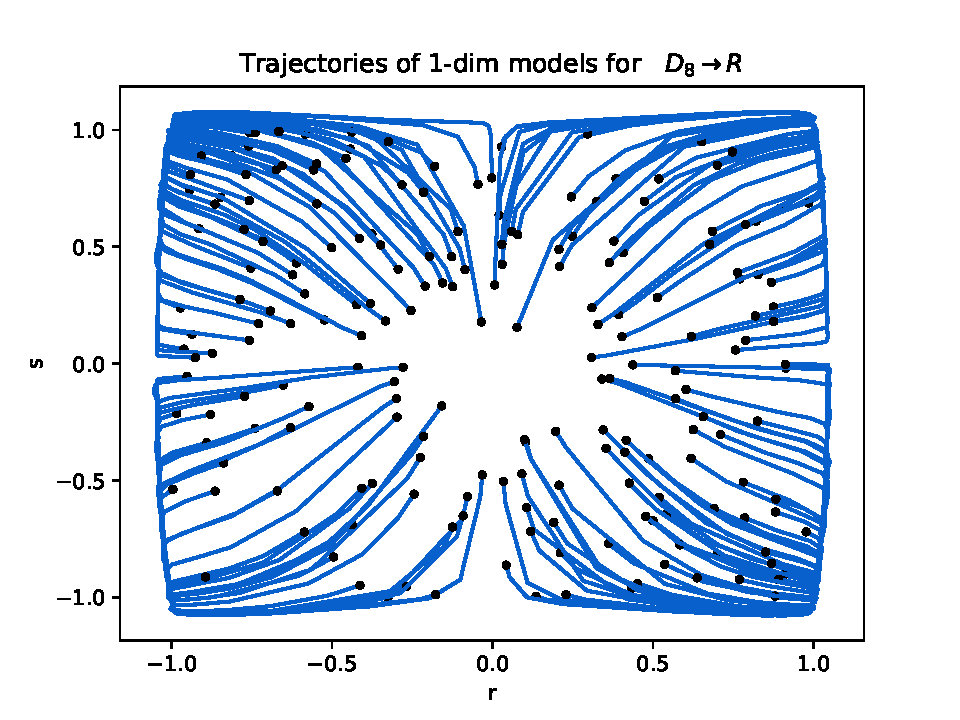
\includegraphics[width=\linewidth]{images/dihedral/Dn_1dim_n8.pdf}
                            \caption*{$n=8$}
                        \end{minipage} 
            \caption[Rešitve enačb gradientnega toka za različne $n$ in različne začetne parametre. Črne pike predstavljajo začetne vrednosti rešitev. Modre rešitve kovergirajo k nerazcepni upodobitvi, oranžne pa v lokalni minimum $\loss$, ki ni globalni. 
Več grafov je v \TODO{Dodatek}.]{Rešitve enačb gradientnega toka za različne $n$ in različne začetne parametre\footnote{Na vsakem grafu je 200 različnih rešitev. Začetni parametri so vzorčeni iz enakomerne porazdelitve nad $[-1,1]^2$. Za implementacijo glej \TODO{implementacija}}. 
Črne pike predstavljajo začetne vrednosti rešitev. Modre rešitve kovergirajo k nerazcepni upodobitvi, oranžne pa v lokalni minimum $\loss$, ki ni globalni. 
Več grafov je v \TODO{Dodatek}.}
            \label{fig:Dn-trajektorije-demo}
        \end{figure}
% 
% 
% 
        Opazimo, da vse numerične rešitve z začetnimi parametri $(r_0, s_0)$ konvergirajo k $\operatorname{sign}(r_0), \operatorname{sign}(s_0)$. Za vsak par začetnih parametrov $(r_0, s_0) \in \R^2$ enodimenzionalnega modela lahko študiramo hitrost konvergence h lokalnim ekstremom. Slika 
        \TODO{} prikazuje čas $t_{r_0, s_0}$, ob katerem je rešitev $(r(t), s(t))$ z začetnimi parametri $(r_0, s_0)$ prvič v $\epsilon = TODO$ pasu njene limite v neskončnosti. 
        \begin{figure}[h!]
            \centering
            \includegraphics[width=0.8\linewidth]{images/dihedral/grid/plot_dihedral_grid_n4_-3_3_1000.pdf}
            \caption{Hitrosti konvergenc različnih začetnih parametrov. Barva točke $(r_0,s_0)$ določa limito - zelene točke konvergirajo k $(1,1)$, modre k $(1,-1)$, oranžne k $(-1,-1)$ in rdeče k $(-1,1)$. Odtenek točke določa hitrost konvergence rešitve $(r(t), s(t))$. Svetlejša, kot je barva, manjši je prvi $t_1$, v katerem se $(r(t_1), s(t_1))$ razlikuje od limite za manj kot $\epsilon = 0.01$.}
            \label{fig:enter-label}
        \end{figure}
        \subsubsection{Dvodimenzionalne upodobitve}
        Model dvorazsežne upodobitve $D_n$ je določen z matrikama $\hat \rho(s) = S \in \R^{2\times 2}$ in $\hat \rho(r) = R \in \R^{n \times n}$. Funkcije izgube so enake 
        \begin{align*}
            \Loss{rel} &= \frac{1}{3} \left( ||S^2 -1||_F^2 + ||R^n -1||_F^2  + ||(RS)^2 -1||_F^2  \right )\\
            \Loss{unit} &=  \frac{1}{2} \left ( ||R^2 -1||_F^2 + ||S ^2 -1||_F^2  \right)  \\
            \Loss{irr} &= \left ( \frac{1}{2n}\sum_{i=0}^n(||R^i||_F^2 + ||R^iS||_F^2)    - 1\right )^2.
        \end{align*}
        \paragraph{Numerične rešitve} 
        Slika \TODO prikazuje numerične rešitve za različne začetne parametre. Trajektorije rešitev $(R(t), S(t))$ vizualiziramo v $\R^2$ kot $(\operatorname{tr}(R(t), \operatorname{tr(S(t)})$. 
        \begin{figure}[h!]
            \centering
                      \begin{minipage}{0.49\textwidth}
                            \centering
                            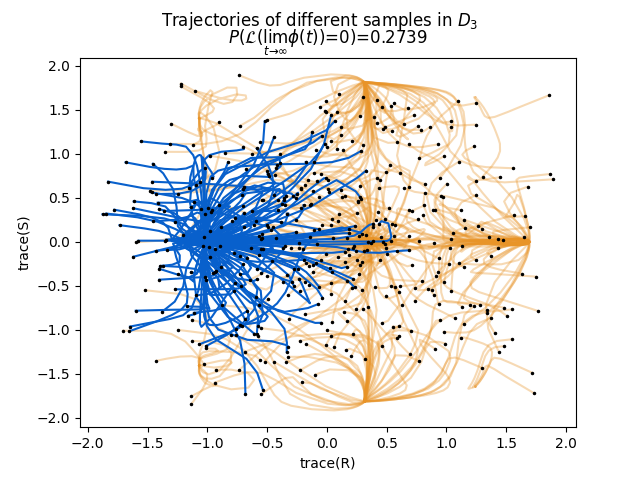
\includegraphics[width=\linewidth]{images/dihedral/2d/prob_of_convergence_D_3.png}
                            \caption*{$n=3$}
                        \end{minipage} 
                    \begin{minipage}{0.49\textwidth}
                            \centering
                            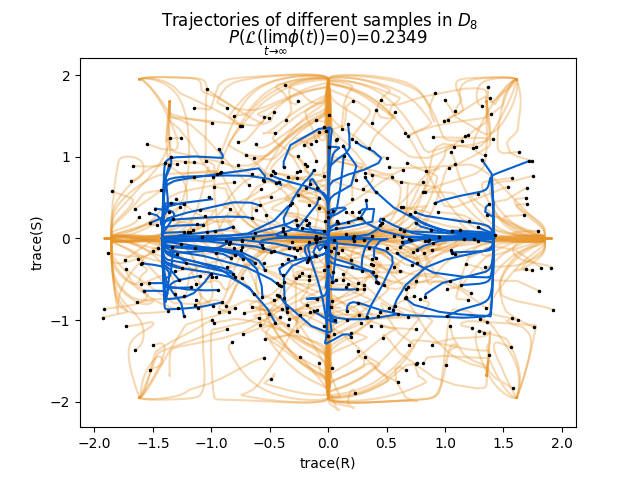
\includegraphics[width=\linewidth]{images/dihedral/2d/prob_of_convergence_D_8.png}
                            \caption*{$n=8$}
                        \end{minipage} 
            \caption[Rešitve za različne $n$. Modre krivulje konvergirajo do nerazcepnih upodobitev. Črne pike so začetni parametri]{Rešitve za različne $n$. Modre krivulje konvergirajo do nerazcepnih upodobitev. Črne pike so začetni parametri\footnotemark
            % \footnote{Začetni parametri $R_0, S_0 $ so oblike $\begin{bmatrix}
            %     x & y \\
            %     z & \operatorname{tr} - x
            % \end{bmatrix}$, kjer so $x,y,z, \operatorname{tr} \sim U[-2,2]$}
            .}
            \label{fig:diederska-2dim-trajektorije}
        \end{figure}
        \footnotetext{Začetni parametri $R_0, S_0 $ so oblike $\begin{bmatrix}
                x & y \\
                z & \operatorname{tr} - x
            \end{bmatrix}$, kjer so $x,y,z, \operatorname{tr} \sim U[-2,2]$}
        Nekateri začetni parametri vodijo do nerazcepne upodobitve, drugi ne. Računamo lahko verjetnost izbire začetnih parametrov, ki konvergirajo do ničel funkcije izgube. Verjetnosti v tabeli \ref{tab:verjetnost-konvergence-diederska-2dim} so izračunane iz iz vzorcov v dodatku \TODO.  
        \begin{table}[ht]
    \centering
    \begin{tabular}{c|c}
         Group &  $P\left( \loss (\lim \limits_{t \to \infty}\phi(t)) = 0  \right)$\\
         \hline
$D_{3}$ & $0.274$\\
$D_{4}$ & $0.158$\\
$D_{5}$ & $0.306$\\
$D_{6}$ & $0.21$\\
$D_{7}$ & $0.311$\\
$D_{8}$ & $0.235$\\
$D_{9}$ & $0.33$\\
$D_{10}$ & $0.241$\\
$D_{11}$ & $0.327$\\
$D_{12}$ & $0.248$\\
$D_{13}$ & $0.319$
    \end{tabular}
    \caption{Verjetnost izbire začetnih parametrov, ki konvergirajo. Začetni parametri so vzorčeni enako kot v \ref{fig:diederska-2dim-trajektorije}. Velikost vzorca je $10^4$.}
    \label{tab:verjetnost-konvergence-diederska-2dim}
\end{table}
        %%%%%%%%%%%%%%%%%%%%%%%%%
        %%%%%%%%%%%%%%%%%%%
        \subsection{Parametrizacija ortogonalne grupe}
        \TODO{Študiramo $p \colon \R \to O_2$}.
% %%%%%%%%%%%%%%%%%%%%%%
% %%%%%%%%%%%%%%%%%%
% %%%%%%%%%%%%%%%%%%%%%%%%%
% %%%%%%%%%%%%%%%%%%%%%%%%%%%%%%%%%%%%%
% //////////////////////
%%%%%%%%%%%%%%%%%%%%%%%%%%
%%%%%%%%%%%%%%%%%%%%%%%%%%%%
\clearpage%newpage pusti floatom, da so prej!
\section{Iskanje delovanj}
Na podoben način lahko iščemo delovanja grup. Naj bo $G$ končna grupa in $[n] =    \{1,2,\dotsc, n\}$ končna množica. Iščemo homomorfizem $\rho \colon G \to S_n$.

Vsako preslikava $f \in \funnn{n}$ se da predstaviti z vektorjem $\begin{bmatrix}
    f(1)\\
    \vdots \\
    f(n)
\end{bmatrix} \in \R^n$. Lahko bi začeli s poljubno preslikavo $\hat \rho \colon S \to \R^n$ in sistematično spreminjali elemente vektorjem $\hat\rho(s)$, dokler ne pridemo do homomorfizma. To se da, a za optimizacijo parametrov ne moremo uporabiti gradientnega spusta, saj je prostor vektorjev $\{[f(i)]_{i=1, \dotsc n} | f \in \funnn{n}\}$ diskreten. 

 V strojnem učenju nad diskreten prostor izidov $D$ običajno definiramo gladko družino porazdelitev $\{\mathcal{P}_\phi(D)\}$ in minimiziramo  $-\log(P_\phi (\text{opaženi izidi}))$. 
 
 Nad prostorom funkcij $\funnn{n}$ definiramo gladko družino porazdelitev. Generatorje grupe sprva slikamo v poljubne porazdelitve, nato pa spreminjamo porazdelitve, da je verjetnost za homomorfizem čim večja.

 Model $\hat \rho$ delovanja $\rho \colon G \to S_n$ bo preslikava $\hat \rho \colon G \to \mathcal{P}(\funnn{n})$, definirana na generatorjih $s \in S$ s predpisom
 \begin{equation}
     \label{eq: model za delovanja}
     s \mapsto \begin{bmatrix}
        P(s(1) = 1) & P(s(1) = 2) & \dotsm & P(s(1) = n) \\
        P(s(2) = 1) & P(s(2) = 2) & \dotsm & P(s(2) = n) \\
        \vdots & \vdots & & \vdots \\
        P(s(n) = 1) & P(s(n) = 2) & \dotsm & P(s(n) = n) \\
    \end{bmatrix}
 \end{equation}
 in implicitno (glej enačbo  \eqref{eq: implicitna definicija upodovbitve}) drugje. Matrika $P_s = \hat\rho(s)$ definira slučajno preslikavo\footnote{Tukaj izrabimo notacijo in s $s$ označimo tako generator  kot slučajno funkcijo nad $[n]$, ki je porazdeljena s porazdelitvijo $P(s = f) = \prod _{i=1}^n P(s(i) = f(i)$. Prav tako za poljuben element $g=s_1s_2\dotsm s_m \in G$ z $g$ označimo tudi slučajno spremenljivko $s_1 s_2 \dotsm s_n$.}
 $s \in \funnn{n}$ s porazdelitvijo 
 $$P(s = f) = \prod _{i=1}^n P(s(i) = f(i)$$ 
 za $f \in \funnn{n}$.

Lahko je preveriti, da za  $g = s_1 s_2 \dotsm s_m\in G$ velja $$
\hat \rho (g) = P_{s_1} P_{s_2} \dotsc P_{s_m} = \begin{bmatrix}
            P(g(1) = 1) & P(g(1) = 2) & \dotsm & P(g(1) = n) \\
        P(g(2) = 1) & P(g(2) = 2) & \dotsm & P(g(2) = n) \\
        \vdots & \vdots & & \vdots \\
        P(g(n) = 1) & P(g(n) = 2) & \dotsm & P(g(n) = n) \\
\end{bmatrix}.
$$ 
Naš model elemente grupe slika v stohastične matrike, ki definirajo verjetnostne porazdelitve slučajnih funkcij nad $n$. Parametre modela bomo optimizirali tako, da bo homomorfizem najbolj verjeten.
\subsection{Parametrizacija stohastičnih matrik}
\label{section:parametrizacija stohastičnih matrik}
Definicija modela $\hat  \rho$ zahteva, da so matrike  $P_s$ stohastične\footnote{$P$ je stohastična, če je vsota elementov v vsaki vrstici enaka $1$, vsi elementi matrike pa so med $0$ in $1$.}. Iteracije gradientnega spusta stohastičnosti ne ohranjajo. Če hočemo za optimizacijo modela $\hat \rho$ uporabiti gradientni spust, moramo metodo prilagoditi tako, da novi parametri ostanejo v družini stohastičnih matrik. 

Družino stohastičnih matrik lahko parametriziramo s poljubno parametrizacijo $p \colon \R^{n \times n} \to \{P \in \R^{n \times n} \mid P \text{ je stohastična }\}$, stohastične matrike $P_s$ pa definiramo kot $p(\phi_s)$, kjer je $\phi = \{\phi_s | s\in S \} \subset \R^{n \times n}$ množica poljubnih matrik. \emph{Za parametre modela} vzamemo elemente matrik $\phi_s$. Na ta način bodo matrike $P_s = P_s(\phi_s)$ vedno stohastične, ne glede na spremembo parametrov $-\eta \nabla_\phi \loss(P)$.

Za parametrizacijo $p$ lahko vzamemo preslikavo $\operatorname{softmax}$, ki vsako vrstico spremeni v stohastični vektor.
\begin{definicija}
     Preslikava $\operatorname{softmax} \colon \R^n \to \R^n$ slika vektor $v = [v_1, v_2, \dotsc, v_n]^T$ v vektor z elementi $\operatorname{softmax}(v)_i = \frac{e^{v_i}}{\sum_{j = 1}^n e^{v_j}}$.

     Za matriko $A = \begin{bmatrix}
         a_1^T \\ 
         a_2^T \\ 
         \vdots \\ 
         a_n^T
     \end{bmatrix}$ definiramo \emph{softmax po vrsticah} kot 
     $$\operatorname{softmax}(A) = \begin{bmatrix}
         \operatorname{softmax}(a_1)^T \\ 
         \operatorname{softmax}(a_2)^T \\ 
         \vdots \\ 
         \operatorname{softmax}(a_n)^T
     \end{bmatrix}.$$
\end{definicija}
Preslikava $\operatorname{softmax}$ očitno poljubne matrike preslika v stohastične. Z njo lahko za generator $s \in S$ matriko $P_s$ definiramo kot 
$$
P_s = \operatorname{softmax}(\phi_s).
$$
Model za delovanja $\hat \rho = \hat \rho_\phi$ definiramo v odvisnosti od parametrov $\phi = \{\phi_s \in \R^{n \times n } \mid s \in S\}$ kot 
$$
\phi \mapsto ( s \mapsto \operatorname{softmax}(\phi_s))
$$
in spreminjamo elemente matrik $ \phi_s$, da model $\hat \rho_\phi$ skoraj zagotovo predstavlja delovanje. 

\subsection{Funkcija izgube nad relacijami}
Naj bo $<S|R>$ prezentacija grupe $G$. Za vsako relacijo $r \in R$ bi radi $P(r = \operatorname{id}) =1$ oziroma $0 = \log(P(r=\operatorname{id})) = \log(\prod_{i=1}^n P(r(i)=i)) = \operatorname{tr}(\log(P_r))$, kjer $\log(P_r)$ računamo po elementih. 
\begin{definicija}
    \emph{Funkcijo izgube nad relacijami} za delovanja definiramo kot 
    \begin{equation}
        \label{eq:relation loss actions}
        \Loss{rel} (\hat\rho) = - \frac{1}{|R|} \sum_{r \in R} \operatorname{tr}(\log(P_r)).
    \end{equation}
\end{definicija}
\subsection{Pretvorba modela v delovanje}

\subsection{Delovanje ciklične grupe}
Študiramo model za delovanje ciklične grupe $C_n = <z | z^n=1>$ na končni množici $[m] = \{1,2,\dotsc, m\}$. Minimaliziramo
$$
\loss(\phi) = - \operatorname{tr}(\log (\operatorname{softmax}(\phi))),
$$
kjer je $\phi \in \R^{m \times m}$.
\paragraph{Rezultati}
\begin{figure}
    \centering
    \begin{minipage}{0.49\textwidth}
            \centering
            \includegraphics[width=\linewidth]{images/actions/C6_on_6_sample8_initial.pdf}
            \caption*{$n=6, m=6$}
        \end{minipage} 
        \begin{minipage}{0.49\textwidth}
            \centering
            \includegraphics[width=\linewidth]{images/actions/C6_on_6_sample8_final.pdf}
            \caption*{Model konvergira k $(154)(236)$.}
        \end{minipage} 
    \caption[Stohastične matrike na začetku in po \TODO korakih gradientnega spusta.]{Stohastične matrike na začetku in po \TODO korakih gradientnega spusta\footnote{\TODO kaka implementacija}.}
    \label{fig:actions-cn}
\end{figure}
\TODO{dodaj slike in rezultate}
\subsection{Rekurzivni pristop}

\TODO{DOdaj rekurzivni (strojnoučenjaški) pristop. Potestiraj ga}

\section{Iskanje izomorfizmov grafov}
S podobnim pristopom kot v \ref{eq: repr model na S} lahko iščemo izomorfizme grafov. Iščemo model za bijektivno preslikavo $f \colon G_1 \to G_2$ med grafoma $G_1$ in $G_2$, za katero velja $f(i) \sim_2 f(j) \iff i \sim_1 j$.

Za model lahko vzamemo slučajno preslikavo $f$, podano s stohastično matriko $P_f = \begin{bmatrix}
            P(f(1) = 1) & P(f(1) = 2) & \dotsm & P(f(1) = n) \\
        P(f(2) = 1) & P(f(2) = 2) & \dotsm & P(f(2) = n) \\
        \vdots & \vdots & & \vdots \\
        P(f(n) = 1) & P(f(n) = 2) & \dotsm & P(f(n) = n) \\
\end{bmatrix} $ in spreminjamo elemente matrike tako, da je $f $ vse bolj verjetno izomorfizem. Zato potrebujemo funkcijo izgube, ki je ničelna natanko v izomorfizmih - torej bijektivnih preslikavah, ki slikajo povezane vozlišča v povezane. 
\subsection{Funkcija izgube za bijektivnost}
Naj bo $f$ slučajna preslikava iz $\funnn{n}$, definirana kot zgoraj. Radi bi, da je $f$ skoraj zagotovo bijektivna, torej da velja 
\begin{align*}
    1 &= P(f \in S_n) \\
    &= \sum_{\sigma  \in S_n} P(f =  \sigma) \\
    &= \sum_{\sigma  \in S_n} \prod_{i=1}^n (P_f)_{i, \sigma(i)} \\
    &= \operatorname{Perm(P_f)},
\end{align*}
kjer $\operatorname{Perm}(P_f)$ označuje \emph{permanent} \footnote{$\operatorname{Perm}(A) = \sum_{\sigma  \in S_n} \prod_{i=1}^n A_{i, \sigma(i)}$} matrike $P_f$.

Za stohastične matrike velja spodnja lema.
\begin{lema}
    Za stohastično matriko $P$ velja $\operatorname{Perm}(P)=1$ natanko tedaj, ko je $P$ permutacijska.
\end{lema}
\begin{dokaz}
    Če je $P$ permutacijska, ima očitno enotski permanent. Dokažimo lemo še v obratno smer.
    
    Naj bo $P = \begin{bmatrix}
        p_{i,j}
    \end{bmatrix}_{i,j=1,\dotsc, n}$ poljubna stohastična matrika s $\operatorname{Perm}(P) = 1$. Po definicijo so vsi elementi  $p_{i,j}$ matrike med $0$ in $1$, vrstice se pa seštejejo v $1$.
    Velja
    $$
    \operatorname{Perm}(P) = \sum_{\sigma  \in S_n} \prod_{i=1}^n p_{i, \sigma(i)} \leq \sum_{\sigma  \in \funnn{n}} \prod_{i=1}^n p_{i, \sigma(i)},
    $$
    saj so vsi elementi stohastične matrike nenegativni, in smo vsoti zgolj prišteli nenegativne elemente.

    Vsako funckijo $\sigma \in \funnn{n}$ lahko predstavimo z vektorjem $(\sigma_1, \sigma_1, \dotsc, \sigma_n)$, kjer je $\sigma_i = \sigma(i) \in \N$. Tako je 
    $$
    \sum_{\sigma  \in \funnn{n}} \prod_{i=1}^n p_{i, \sigma(i)} =
    \sum_{(\sigma_1, \sigma_1, \dotsc, \sigma_n) \in [n]^n} \prod_{i=1}^n p_{i, \sigma_i} = 
    \prod_{i=1}^n (p_{i, 1} + p_{i, 2} + \dotsm + p_{i, n}).
    $$
    Ker so vsote vrstic enake $1$, velja 
    $$
    1 = \operatorname{Perm}(P) \leq  \sum_{\sigma  \in \funnn{n}} \prod_{i=1}^n p_{i, \sigma(i)} = \prod_{i=1}^n (p_{i, 1} + p_{i, 2} + \dotsm + p_{i, n}) = 1.
    $$
    Sledi, da je  $\sum_{\sigma  \in S_n}  \prod_{i=1}^n p_{i, \sigma(i)} =  \sum_{\sigma  \in \funnn{n}} \prod_{i=1}^n p_{i, \sigma(i)} $ in posledično je vsota 
    $ 
    \sum_{\sigma  \in \funnn{n} \setminus S_n} \prod_{i=1}^n p_{i, \sigma(i)}
    $ enaka $0$.

    Zdaj lahko dokažemo, da je  v poljubnem stolpcu matrike $P$ lahko največ en ne-ničelni element. Naj bo $i$ indeks poljubnega stolpca in $r \neq s$ indeksa dveh vrstic. Recimo, da sta elementa $p_{r, i}$ in $p_{s,i}$ oba neničelna. 

    Definiramo lahko tako preslikavo $f \in \funnn{n}$, da je $f(r) = f(s) = i$, za $j \notin \{r, s\}$ pa $f(j)$ izberemo tako, da $p_{j, f(j)}$ ni ničelen (to lahko vedno izberemo, saj je matrika stohastična, torej ima v vsaki vrstici vsaj en neničelen element). 

    Očitno je $\prod_{i=1}^n p_{i, f(i)} \neq 0$, kar pa je v protislovju z $ \displaystyle \sum_{\sigma  \in \funnn{n} \setminus S_n} \prod_{i=1}^n p_{i, \sigma(i)}$.   V vsakem stolpcu matrike je torej natanko en neničelen element. 

    Velja še $1 = P(f \in S_n) = P(f \text{ je surjektivna}) = \prod_{i=1}^n P(\exists j \in \N. f(j)= i) = 
     \prod_{i=1}^n (\sum_{j=1}^n p_{j, i})$, torej se vsote stolpcev zmnožijo v $1$. Ker je v vsakem stolpcu natanko en neničelen element sledi, da je ta element enak $1$.  Posledično je tudi v vsaki vrstici natanko en neničelen element (sicer se vrstica ne bi seštela v $1$), kar pomeni, da je $P$ permutacijska. 
\end{dokaz}
Slučajna preslikava $f$ je torej skoraj zagotovo bijektivna natanko tedaj, ko je $P_f$ permutacijska. Enostavno je preveriti, da so stohastične matrike permutacijske natanko tedaj, ko so unitarne. Bolj, kot bo $P_f$ unitarna, bolj verjetno bo $f$ bijektivna. 

Če $P_f$ definiramo kot 
$$P_f = \operatorname{softmax}(\phi)$$(glej poglavje \ref{section:parametrizacija stohastičnih matrik}), lahko za funkcijo izgube vzamemo $\phi \mapsto \Loss{unitary}(P_f)$. 

\begin{definicija}
    Za poljubno realno matriko $\phi \in \R^{n \times n}$ \emph{funkcijo izgube za bijektivnost} definiramo kot 
    $$
    \Loss{bijective} = \Loss{unitary} \circ \operatorname{softmax}.
    $$
\end{definicija}
Z minimiziranjem iste funkcije izgube lahko rešujemo dva različna problema (problem iskanja unitarnih matrik in problem iskanja bijekcij) preslikava $\operatorname{softmax}$  pa pretvarja med problemoma. 
\subsection{Funkcija izgube za povezanost}
    Naj bosta $G_1 = ([n], E_1)$ in $G_2 = ([n], E_2)$ grafa  in $M_1, M_2$ njuni matriki sosednosti. 
    Za $i \sim_1 j$ bi radi, da je $P(f(i)  \sim_2 f(j)) = 1$.
    Računamo 
    $$
    P(f(i) \sim_2 f(j)) = \sum_{k= 1}^n \sum_{h = 1}^n p_{i, k} p_{j, h} m_{k,h}^{(2)} 
% = f_j^T M_1 f_i
= (P M_2 P^T)_{i, j}
    $$
    \begin{definicija}
        \emph{Funkcijo izgube za povezanost}\footnote{$\log$ računamo po elementih}. lahko izpeljemo kot 
        \begin{align*}
    \mathcal{L}_\sim &= -\sum_{i \sim_1 j} \log P(f(i) \sim_2 f(j)) 
    \\&= -\sum_{i=1}^n\sum_{j=1}^n log(f_j^T M_2 f_i)m_{i,j}^{(1)}\\&= -\operatorname{tr}(\log(P_fM_2P_f^T) M_1^T). 
\end{align*}
    \end{definicija}
\subsection{Rezultati}
\begin{primer}
    Poglejmo si preprost graf \ref{fig:primer_grafa} na petih točkah $\{0,1,2,3,4\}$, s povezavami $\{0 \sim 4, 4 \sim 3, 3 \sim 0, 3 \sim 1, 2 \sim 0\}$. Očitno je grupa avtomorfizmov tega grafa izomorfna diedrski grupi trikotnika $D_3$. 
    \begin{figure}[h!]
        \centering
        \includegraphics[width=0.5\linewidth]{images/random_samples_big_random_graph_1_on_5.png}
        \caption{Graf na petih vozljiščih.}
        \label{fig:primer_grafa}
    \end{figure}
    
       Gradientni spust poleg trivialne rešitve na določenih začetnih parametrih uspe najti avtomorfizem $(03)(24)$, na drugih pa konvergira do limite, ki ni blizu avtomorfizma. 
    
\end{primer}

Rezultati simulacij nad različnim cayleyevim igrafi so v \ref{dodatek:cayley},
nad različnimi naključno tvorjenimi grafi pa v  \ref{dodatek:naključni grafi}.
 
\section{Preparametrizacije}
\TODO{overparmetrisations}

\section{Dodatek}
\subsection{Izomorfizmi Cayleyevih grafov}
\label{dodatek:cayley}
\includepdf[pages=-]{pdfs/aut_calyey.pdf}

         


 \subsection{Izomorfizmi naključnih grafov}
\label{dodatek:naključni grafi}
\TODO{Sem gredo dodatki, dodatni doakzi, itd..}
\subsection{Dovolj so upodobitve nad končnimi množicami}
    




% \section{Integrali po \texorpdfstring{$\omega$}{ω}-kompleksih}
% \subsection{Definicija}
% \begin{definicija}
%   Neskončno zaporedje kompleksnih števil, označeno z $\omega = (\omega_1, \omega_2, \ldots)$,
%   se imenuje \emph{$\omega$-kompleks}.\footnote{To ime je izmišljeno.}

%   Črni blok zgoraj je tam namenoma. Označuje, da \LaTeX{} ni znal vrstice prelomiti pravilno
%   in vas na to opozarja. Preoblikujte stavek ali mu pomagajte deliti problematično besedo z
%   ukazom \verb|\hyphenation{an-ti-ko-mu-ta-ti-ven}| v preambuli.
% \end{definicija}
% \begin{trditev}[Znano ime ali avtor]
%   \label{trd:obstoj-omega}
%   Obstaja vsaj en $\omega$-kompleks.
% \end{trditev}
% \begin{proof}
%   Naštejmo nekaj primerov:
%   \begin{align}
%     \omega &= (0, 0, 0, \dots), \label{eq:zero-kompleks} \\
%     \omega &= (1, i, -1, -i, 1, \ldots), \nonumber \\
%     \omega &= (0, 1, 2, 3, \ldots). \nonumber \qedhere  % postavi QED na zadnjo vrstico enačbe
%   \end{align}
% \end{proof}

% \section{Tehnični napotki za pisanje}

% \subsection{Sklicevanje in citiranje}
% Za sklice uporabljamo \verb|\ref|, za sklice na enačbe \verb|\eqref|, za citate \verb|\cite|. Pri
% sklicevanju in citiranju sklicano številko povežemo s prejšnjo besedo z nedeljivim presledkom
% $\sim$, kot npr.\ \verb|iz trditve~\ref{trd:obstoj-omega} vidimo|.

% \begin{primer}
%   Zaporedje~\eqref{eq:zero-kompleks} iz dokaza trditve~\ref{trd:obstoj-omega} na
%   strani~\pageref{trd:obstoj-omega} lahko najdemo tudi v Spletni enciklopediji zaporedij~\cite{oeis}.
%   Citiramo lahko tudi bolj natančno~\cite[trditev 2.1, str.\ 23]{lebedev2009introduction}.
% \end{primer}

% \subsection{Okrajšave}
% Pri uporabi okrajšav \LaTeX{} za piko vstavi predolg presledek, kot npr. tukaj. Zato se za vsako
% piko, ki ni konec stavka doda presledek običajne širine z ukazom \verb*|\ |, kot npr.\ tukaj.
% Primerjaj z okrajšavo zgoraj za razliko.

% \subsection{Vstavljanje slik}
% Sliko vstavimo v plavajočem okolju \texttt{figure}. Plavajoča okolja \emph{plavajo} po tekstu, in
% jih lahko postavimo na vrh strani z opcijskim parametrom `\texttt{t}', na lokacijo, kjer je v kodi s
% `\texttt{h}', in če to ne deluje, potem pa lahko rečete \LaTeX u, da ga \emph{res} želite tukaj,
% kjer ste napisali, s `\texttt{h!}'. Lepo je da so vstavljene slike vektorske (recimo \texttt{.pdf}
% ali \texttt{.eps} ali \texttt{.svg}) ali pa \texttt{.png} visoke resolucije (več kot
% \unit[300]{dpi}).  Pod vsako sliko je napis in na vsako sliko se skličemo v besedilu. Primer
% vektorske slike je na sliki~\ref{fig:sample}. Vektorsko sliko prepoznate tako, da močno
% zoomate v sliko, in še vedno ostane gladka. Več informacij je na voljo na
% \url{https://en.wikibooks.org/wiki/LaTeX/Floats,_Figures_and_Captions}. Če so slike bitne, kot na
% primer slika~\ref{fig:image}, poskrbite, da so v dovolj visoki resoluciji.

% \begin{figure}[h]
%   \centering
%   \includegraphics[width=0.6\textwidth]{images/sample.pdf}
% % \caption[caption za v kazalo]{Dolg caption pod sliko}
%   \caption[Primer vektorske slike.]{Primer vektorske slike z oznakami v enaki pisavi, kot jo
%      uporablja \LaTeX{}.  Narejena je s programom Inkscape, \LaTeX{} oznake so importane v
%      Inkscape iz pomožnega PDF.}
%   \label{fig:sample}
% \end{figure}

% \begin{figure}[h]
%   \centering
%   \includegraphics[width=0.8\textwidth]{images/image.png}
%   \caption[Primer bitne slike.]{Primer bitne slike, izvožene iz Matlaba. Poskrbite, da so slike v
%   dovolj visoki resoluciji in da ne vsebujejo prosojnih elementov (to zahteva PDF/A-1b format).}
%   \label{fig:image}
% \end{figure}

% \subsection{Kako narediti stvarno kazalo}
% Dodate ukaze \verb|\index{polje}| na besede, kjer je pojavijo, kot tukaj\index{tukaj}.
% Več o stvarnih kazalih je na voljo na \url{https://en.wikibooks.org/wiki/LaTeX/Indexing}.

% \subsection{Navajanje literature}
% Članke citiramo z uporabo \verb|\cite{label}|, \verb|\cite[text]{label}| ali pa več naenkrat s
% \verb|\cite\{label1, label2}|. Tudi tukaj predhodno besedo in citat povežemo z nedeljivim presledkom
% $\sim$. Na primer~\cite{chen2006meshless,liu2001point}, ali pa \cite{kibriya2007empirical}, ali pa
% \cite[str.\ 12]{trobec2015parallel}, \cite[enačba (2.3)]{pereira2016convergence}.
% Vnosi iz \verb|.bib| datoteke, ki niso citirani, se ne prikažejo v seznamu literature, zato jih
% tukaj citiram.~\cite{vene2000categorical}, \cite{gregoric2017stopniceni}, \cite{slak2015induktivni},
% \cite{nsphere}, \cite{kearsley1975linearly}, \cite{STtemplate}, \cite{NunbergerTand}, \cite{vanoosten2008realizability}.

\end{document}
